\documentclass[12pt,letterpaper]{article}
\usepackage{amsmath,amsthm,amsfonts,amssymb,amscd}
\usepackage{listings}
\usepackage{color}
\usepackage{MnSymbol,wasysym}
\usepackage{caption}
\usepackage{subcaption}

\definecolor{dkgreen}{rgb}{0,0.6,0}
\definecolor{gray}{rgb}{0.5,0.5,0.5}
\definecolor{mauve}{rgb}{0.58,0,0.82}

\lstset{%frame=tb,
  language=Bash,
  aboveskip=3mm,
  belowskip=3mm,
  showstringspaces=false,
  columns=flexible,
  basicstyle={\small\ttfamily},
  numbers=none,
  numberstyle=\tiny\color{gray},
  keywordstyle=\color{black},%blue
  commentstyle=\color{dkgreen},
  stringstyle=\color{black},
  breaklines=true,
  breakatwhitespace=true
  tabsize=3
}


\usepackage{hyperref}
\usepackage{graphicx}
\usepackage{enumerate}
\usepackage{fancyhdr}
\usepackage{mathrsfs}
\usepackage[margin=3cm]{geometry}
\setlength{\parindent}{0.0in}
\setlength{\parskip}{0.05in}

% Edit these as appropriate
\newcommand\course{CS595}
\newcommand\semester{Fall 2013}     
\newcommand\hwnum{9}
\newcommand\yourname{Mohamed Aturban}
\newcommand\login{maturban}

\newenvironment{answer}[1]{
  \subsubsection*{Problem #1}
}

\pagestyle{fancyplain}
\headheight 40pt
\lhead{\yourname\ (\login)\\\course\ --- \semester}
\chead{\textbf{\Large Assignment \hwnum}}
\rhead{\today}
\headsep 40pt

\begin{document}

All files mentioned in this document should be uploaded into the {\it github} repository.

\begin{answer}{1: Creating a blog-term matrix}

\begin{itemize}

\item Collecting URIs:

A list of URIs of online blogs has been downloaded from: \url {https://github.com/nico/collectiveintelligence-book}, and stored in a file called {\it feedlist.txt}, then each of these URIs has been validated by the online Atom/RSS feed validation service: \url {http://validator.w3.org/feed/}. The next two figures show, respectively, examples of a valid and invalid Atom/RSS feed:


\begin{figure}[ht!]
\centering
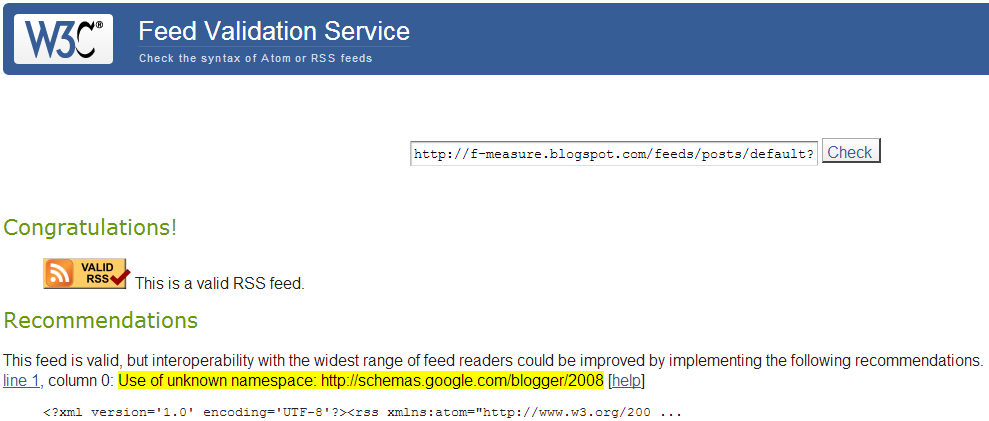
\includegraphics[scale=0.6]{valid}
\caption{Valid Atom/RSS feed URI}
\label{overflow}
\end{figure}

\vspace{5 mm}

\begin{figure}[ht!]
\centering
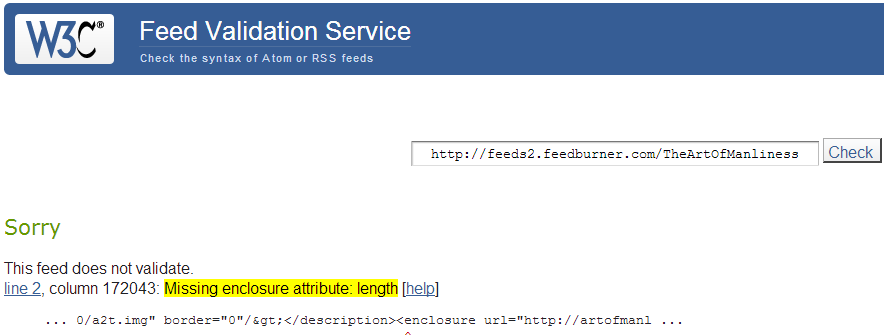
\includegraphics[scale=0.65]{invalid}
\caption{Invalid Atom/RSS feed URI}
\label{overflow}
\end{figure}

The Atom/RSS feed validation service web site indicates that 28, as listed below, out of 100 URIs are not valid feeds; they were replaced by valid Atom/RSS feeds of different blogs.

\begin{lstlisting}[]
	Another examples of invalid Atom/RSS feeds ca-
	ught by the Atom/RSS feed validation service 
	web site
	---------------------------------------------
	http://feeds.feedburner.com/37signals/beMH
	http://featured.gigaom.com/feed/
	http://feeds.feedburner.com/paulstamatiou	   
	http://thinkprogress.org/feed/
	http://www.bloglines.com/rss/about/news
	http://feeds.dailykos.com/dailykos/index.xml
	http://www.downloadsquad.com/rss.xml
	http://www.huffingtonpost.com/raw_feed_index.rdf
	http://www.joelonsoftware.com/rss.xml
	http://feeds.kottke.org/main
	http://www.oilman.ca/feed/
	http://www.powazek.com/rss.xml
	http://www.readwriteweb.com/rss.xml
	...	
\end{lstlisting}

   
The next step now is to run {\it generatefeedvector.py}. This should create a text file called {\it blogdata.txt} which should contain information about the online blogs such as blogs titles` names and words frequencies in each blog. Having 100 valid Atom/RSS feeds does not mean that we will get 100 different blogs titles written in the file {\it blogdata.txt} because different URIs may have the same title. To avoid this, the python code, represented in our textbook, has been modified to print all blogs` URIs that have similar titles. These URIs have been replaced with new Atom/RSS feeds. The following are examples of blogs feeds that have same titles:

\begin{lstlisting}[]
	Blog Title       URI
	----------------------------------------------------
	[Mashable]	http://feeds.feedburner.com/Mashable
	[Mashable]	http://feeds.mashable.com/Mashable
	[The V Spot]	http://www.thevspotblog.com/feeds/posts
				/default?alt=rss
	[The V Spot]	http://feeds.feedblitz.com/TheVSpot					
	...	
\end{lstlisting}

The following is an output sample showing all entities` titles of the blog \url {http://f-measure.blogspot.com/feeds/posts/default?alt=rss}:

\begin{lstlisting}[]
	Entities` titles of the blog "f-measure"
	----------------------------------------------------
	The Beastie Boys - "No Sleep Till Brooklyn" (spotlight)]
	Pink Floyd - "Live At Pompeii" (concert)]
	Negativland - "Live at Lewis's, Norfolk VA, November 21, 1992" (concert)]
	Red Rider - "Lunatic Fringe" (forgotten song)]
	The Green Pajamas - "Kim The Waitress" (forgotten song)]
	The Naked and Famous - "Passive Me, Aggressive You" (LP Review)]
	Rachel Goswell - "Waves Are Universal" (LP Review)]
	The Brains - "Money Changes Everything" (the song remains the same)]
	The Beastie Boys - "The Mix-Up" (LP Review)]
	Houndmouth - "Houndmouth" (LP Review)]
	Husker Du - "Candy Apple Grey" (LP Review)]
	Stanley Jordan - "Stairway to Heaven" (the song remains the same)]
	Discharge - "Protest and Survive" (the song remains the same)]
	Galaxie 500 - "Peel Sessions" (LP Review)]
	My Bloody Valentine - "Loveless" (LP Review)]
	Sonic Youth - "Diamond Sea" (forgotten song)]
	Slayer - "Haunting The Chapel" (LP Review)]
	Hank Williams Jr. - "All My Rowdy Friends (Have Settled Down)" (forgotten song)]
	Unkle - "Do Androids Dream of Electric Beats?" (LP Review)]
	Pink Floyd - "Cymbaline" (forgotten song)]
	The Cribs - "Payola" (LP Review)]
	Dale Watson - "Quick Quick, Slow Slow" (spotlight)]
	The Rave Ups - "Positively Lost Me" (forgotten song)]
	Damian Marley - "Welcome To Jamrock" (spotlight)]
	Mariachi El Bronx - "Cell Mates" (spotlight)]				
	...	
\end{lstlisting}

\item Creating a blog-term matrix

As Dr. Nelson has offered two options to answer question 1, I have chosen the second option: including the item/entry description/summary elements in taking in the terms and then limiting the number of words to the most frequent 500 words. Other small modifications to the code have been made: (1) reducing the total number of terms by picking only terms that are between minimum and maximum percentages 0.2 and 0.4; each percentage is computed by simply taking the ratio of the number of occurrences of a word in all blogs to the total number of blogs, (2) considering only words that consist of at least three characters , and (3)  limiting the number of words to the most frequent 500 words. Blow is a list of the obtained 500 words:

\begin{lstlisting}
  month, did, media, course, hard, try, shows, against, fun, friends,
  once, talk, took, money, during, case, thought, night, home, small,
  far, website, told, change, family, watch, everyone, internet, open,
  play, point, game, google, often, support, under, public, tell, man,
  started, short, state, york, place, number, story, though, looks, 
  behind, probably, several, recent, person, early, become, twitter,
  power, months, four, business, others, share, rather, longer, based,
  almost, hand, thanks, popular, run, music, give, including, someone,
  second, hit, wrote, taking, asked, web, possible, deal, nothing, 
  line, trying, minutes, check, finally, says, must, needs, idea, 
  space, care, service, won, social, buy, until, having, control, via,
  soon, holiday, went, american, anyone, future, america, fact, 
  available, recently, job, according, along, wants, large, photo, 
  easy, comments, everything, anything, favorite, aren, house, 
  important, original, came, known, december, instead, information,
  million, season, released, seen, current, written, black, pretty, 
  him, bad, away, attention, com, simple, create, latest, seems, five,
  problem, building, giving, order, following, wanted, takes, heard,
  data, maybe, interesting, quite, reason, ask, kind, especially, 
  ways, please, reading, screen, however, add, book, page, happy, head,
  worth, facebook, companies, friday, word, earlier, wrong, third, 
  half, name, content, running, feel, john, project, art, currently,
  email, else, whole, thinking, call, piece, users, team, likely,
  version, above, november, pick, process, coming, group, late, gets,
  side, announced, given, turn, system, self, able, amazon, report,
  across, creating, among, tuesday, understand, government, couple,
  mark, question, whether, update, weekend, level, wait, women,
  makes, created, meet, example, links, changes, paper, nbsp,
  special, yourself, store, note, plan, link, hope, stop, stuff, death,
  due, mind, usually, yes, continue, either, fast, posted, below, young,
  woman, entire, saw, hours, experience, six, law, writing, weeks, 
  features, wasn, city, white, added, ones, words, decided, similar, 
  former, ready, party, yesterday, spent, save, lost, works, official,
  sometimes, fans, certain, phone, daily, children, include, cool, sign,
  learned, search, room, history, interview, remember, write, personal,
  happened, related, event, exactly, turned, build, later, face, saying,
  goes, national, article, games, launched, lead, step, although, 
  thousands, north, form, record, videos, single, nice, picture, monday,
  problems, results, follow, outside, school, leave, red, appears, box,
  ahead, completely, taken, sort, learn, beautiful, goal, playing,
  office, perfect, research, health, members, believe, seem, mobile, 
  cover, planning, meant, nearly, photos, questions, source, industry,
  hear, october, role, age, youtube, sound, enjoy, ten, click, access,
  shared, action, tools, market, hold, growing, feature, product,
  president, style, food, books, morning, friend, light, talking,
  close, built, track, points, despite, release, lots, focus, quickly,
  worked, general, reports, technology, center, rest, previous, press,
  security, dead, images, christmas, devices, thanksgiving, percent,
  digital, star, chance, starting, program, device, pay, turns, street,
  design, app, type, science, heart, states, hot, platform, answer, 
  front, term, series, happen, tried, couldn, gives, car, services,
  clear, drive, bring, local, human, edition, result, various,
  received, connection, simply, addition, main, country, moving,
  happens, plus, within, washington, forward, stories, details,
  happening, consider, whose, choice, minute, strong, involved, named, 
  glass, awesome, huge, amazing, lines, fan, move, covered, mean, 
  expect, network, holidays, launch, view, directly, fight, needed,
  haven, matter, apparently, price, particularly, text, movie, key,
  etc, period
\end{lstlisting}


I would like to mention two points here: (1) frequently, when running the file {\it generatefeedvector.py}, each time I get slightly different results. This is due to the information in the online blogs is dynamically changed. In addition to this, some URIs , from 1 to 3, become inactive!

{\it generatefeedvector.py} is uploaded into the repository having my modification to the code to met question 1 requirement. The final blog-term matrix is stored in a text file called {\it blogdata.txt}. 



\end{itemize}
%\begin{itemize}
%\item Creating a blog-term matrix:
%\end{itemize}
\end{answer}

\begin{answer}{2: Creating an ASCII and JPEG dendrogram}

Before starting answering this question, I would like to let you know that I have modified the code of the function {\it pearson()}, page 35 in our text book, based on what this web site suggests: \url {http://www.oreilly.com/catalog/errataunconfirmed.csp?isbn=9780596529321}, but these modifications will cause other functions not work probably (e.g. the produced JPEG will have some strange shapes), so I have decided to use the original code.  

The Python code for solving this question can be found in a file called {\it cluster.py}, uploaded to the GitHub repository. The function {\it readfile()} will read the file {blogdata.txt} and return three objects: the rows names,columns names, and the frequencies. They will be stored, respectively, in variables blognames,words, and data; these data will be clustered based on the similarities between the rows values by using the function {\it pearson()}. This clustering can be done by calling the function {\it hcluster()}. Finally, this clustering can be shown by two different formats:

\begin{itemize}

\item ASCII dendrogram. This can obtained by calling the function {\it printclust()}. Part of this ASCII is presented below. The whole ASCII is uploaded into our GitHub repository in a text file called {\it blogclust.txt}:

\begin{lstlisting}
        -
          Neil Gaiman's Journal
          -
            Web Science and Digital Libraries Research Group
            -
              Business Insider
              -
                Boing Boing
                -
                  Gizmodo
                  -
                    Gothamist
                    -
                      over50feeling40
                      -
                        Jezebel
                        -
                          Wired Top Stories
                          F-Measure
  -
    -
      Marbury
      -
        Gawker
        -
\end{lstlisting}

\item JPEG dendrogram. (the function {\it drawdendrogram} will create a file called {\it blogclust.jpg} which shows how blogs are clustered. See figure 2 below:

\begin{figure}[ht!]
\centering
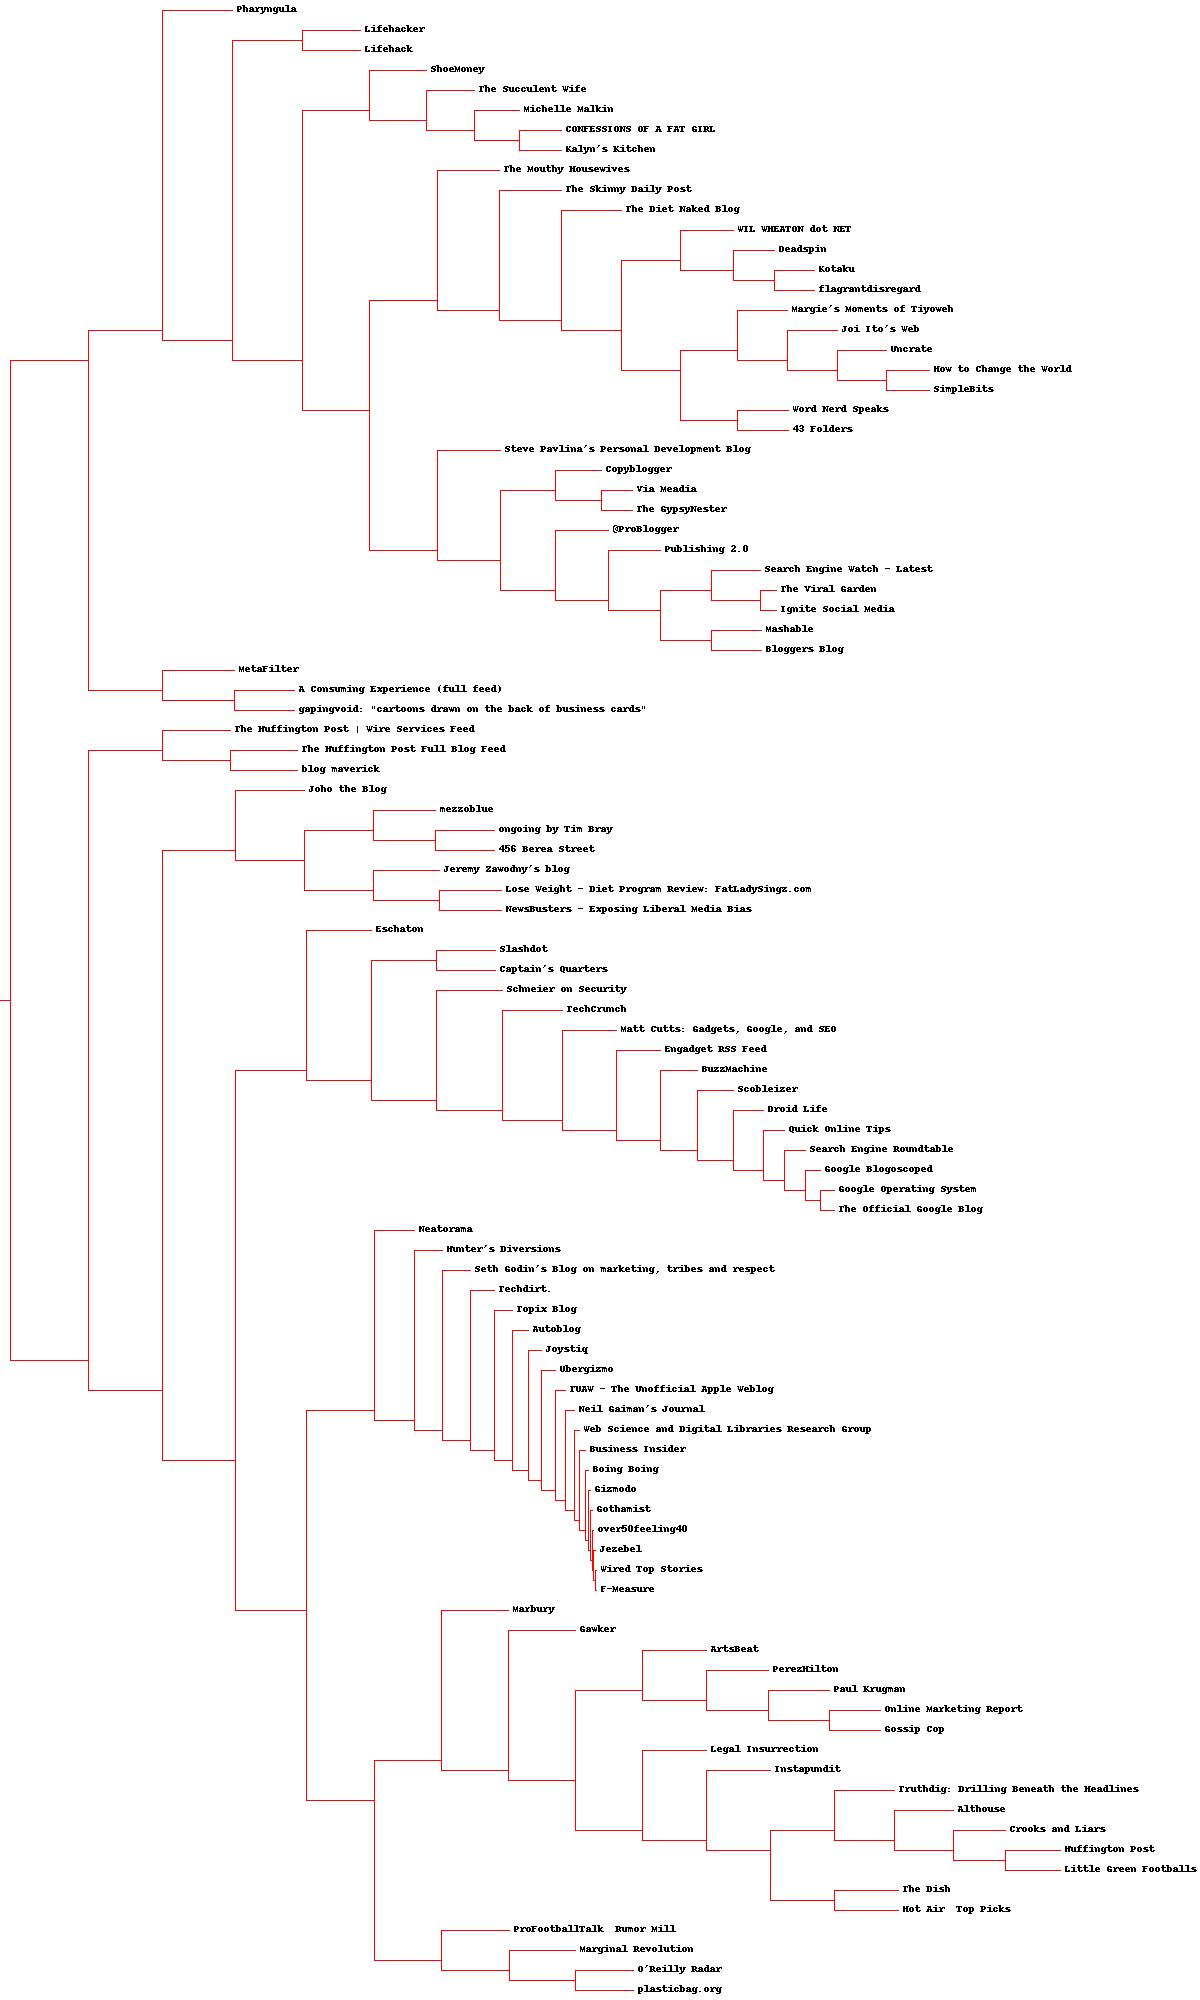
\includegraphics[scale=0.28]{blogclust}
\caption{JPEG dendrogram of the blog clusters}
\label{overflow}
\end{figure}


 
\end{itemize}
   
\end{answer}

\begin{answer}{3: Clustering the blogs using K-Means}

After calling the function {\it kcluster()} with different k values, it returns the following outputs:

\begin{itemize}

\item When k = 5, (it gives the answer after 5 iterations). The following are the 5 clusters:

\begin{lstlisting}
 Cluster 1: 
    ["Neil Gaiman's Journal", 'Web Science and Digital Libraries 
      Research Group', 'Business Insider', 'TUAW - The Unofficial
      Apple Weblog', 'over50feeling40', 'Gizmodo', 'Gothamist',
     'Joystiq', 'Topix Blog', 'Boing Boing', 'Techdirt.', 'Jezebel',
     "Hunter's Diversions", "Seth Godin's Blog on marketing,
      tribes and respect",'Ubergizmo', 'Wired Top Stories',
     'F-Measure', 'Neatorama', 'Autoblog']
 Cluster 2:
    ['Droid Life', '@ProBlogger', 'Search Engine Watch - Latest', 
     'The Dish', "O'Reilly Radar", 'Google Operating System', 
     'Bloggers Blog', 'BuzzMachine', 'flagrantdisregard', 'Scobleizer',
     'Search Engine Roundtable', 'Engadget RSS Feed', 'TechCrunch',
     'A Consuming Experience (full feed)', 'Matt Cutts: Gadgets, 
      Google, and SEO', 'The Official Google Blog', 'Quick Online
      Tips','Google Blogoscoped']
 Cluster 3:
    ['Publishing 2.0', 'Eschaton', 'Word Nerd Speaks', 'Marginal
     Revolution', 'The Succulent Wife', 'Online Marketing Report',
     'Kotaku', 'The Skinny Daily Post', '43 Folders', 'Via Meadia',
     'Deadspin', 'The Huffington Post | Wire Services Feed',
     'CONFESSIONS OF A FAT GIRL', 'Michelle Malkin', 'Lifehacker',
     'SimpleBits', 'ShoeMoney', 'The Diet Naked Blog', 'ProFootballTalk 
      Rumor Mill', 'Copyblogger','PerezHilton', "Kalyn's Kitchen",
      '456 Berea Street', 'Pharyngula', 'The Mouthy Housewives',
      'MetaFilter', 'mezzoblue', 'WIL WHEATON dot NET', 'gapingvoid:
      "car toons drawn on the back of business cards"', 'plasticbag.org',
      'The GypsyNester']
 Cluster 4:
    ['The Huffington Post Full Blog Feed', 'Legal Insurrection',
     'ArtsBeat', 'Mashable', 'Slashdot', 'Instapundit', 
     'ongoing by Tim Bray', 'The Viral Garden', "Captain's Quarters",
     'Ignite Social Media', 'blog maverick', 'Schneier on Security',
     'Huffington Post', "Steve Pavlina's Personal Development Blog",
     'Little Green Footballs', 'Althouse', 'Truthdig: Drilling Beneath
      the Headlines', 'Lifehack', 'Gossip Cop', "Joi Ito's Web",
     'NewsBusters - Exposing Liberal Media Bias', 'Crooks and Liars',
     'Hot Air  Top Picks', 'Gawker', "Margie's Moments of Tiyoweh"]
 Cluster 5:
    ['Lose Weight - Diet Program Review: FatLadySingz.com', 
     'Joho the Blog', 'Uncrate', 'How to Change the World', 'Marbury',
     'Paul Krugman', "Jeremy Zawodny's blog"]
\end{lstlisting}

\item When k = 10, (it gives the answer after 7 iterations). The following are the 10 clusters:

\begin{lstlisting}
 Cluster 1: 
    ["Neil Gaiman's Journal", 'TUAW - The Unofficial Apple Weblog',
     'Joystiq', 'Tech dirt.', "Hunter's Diversions", 'Ubergizmo',
     'Neatorama', 'Autoblog']
 Cluster 2: 
    ['Joho the Blog']
 Cluster 3: 
    ['Publishing 2.0', 'The Huffington Post Full Blog Feed', 
     '@ProBlogger', 'Mashable', 'Bloggers Blog', 'ongoing by
      Tim Bray', 'The Viral Garden', 'Ignite Social Media',
     'blog maverick', 'Schneier on Security', "Steve Pavlina's
      Personal Development Blog", 'Lifehack', "Joi Ito's Web",
     'gapingvoid: "cartoons drawn on the back of business cards"',
     'plasticbag.org', "Margie's Moments of Tiyoweh"]
 Cluster 4: 
    []
 Cluster 5: 
    ['Lose Weight - Diet Program Review: FatLadySingz.com', 
     'Legal Insurrection', 'Via Meadia', 'Instapundit', "Captain's
      Quarters", 'Copyblogger', 'Huffington Post', 'Little Green
      Footballs', 'Althouse', 'Truthdig: Drilling Beneath the 
      Headlines', 'NewsBusters - Exposing Liberal Media Bias',
     'Crooks and Liars', 'Hot Air Top Picks', 'The GypsyNester']
 Cluster 6: 
    ['Word Nerd Speaks', 'Uncrate', 'The Skinny Daily Post',
     'How to Change the World', '43 Folders', 'Lifehacker', 
     'SimpleBits', 'The Diet Naked Blog', '456 BereaStreet',
     'MetaFilter', 'A Consuming Experience (full feed)', 
     'mezzoblue', 'WIL WHEATON dot NET', "Jeremy Zawodny's blog"]
 Cluster 7: 
    ['Marginal Revolution', 'Paul Krugman', 'Pharyngula']
 Cluster 8: 
    ['Eschaton', 'ArtsBeat', 'Online Marketing Report', 'Kotaku',
     'Deadspin', 'The Dish', 'The Huffington Post | Wire Services
      Feed', 'Marbury', 'flagrantdisregard', 'ProFootballTalk  
      Rumor Mill', 'PerezHilton', 'The Mouthy Housewives', 
     'Gossip Cop', 'Gawker']
 Cluster 9: 
    ['Web Science and Digital Libraries Research Group', 
     'Business Insider', 'over50 feeling40', 'Gizmodo', 'Gothamist',
     'Topix Blog', 'Boing Boing', 'Jezebel', "Seth Godin's Blog on
      marketing, tribes and respect", 'Wired Top Stories', 
     'F-Measure']
 Cluster 10: 
    ['The Succulent Wife', 'Droid Life', 'Search Engine Watch 
     - Latest', "O'Reilly Radar", 'CONFESSIONS OF A FAT GIRL',
     'Google Operating System', 'Michelle Malkin', 'ShoeMoney',
     'Slashdot', 'BuzzMachine', 'Scobleizer', 'Search Engine 
      Roundtable', 'Engadget RSS Feed', "Kalyn's Kitchen", 
     'TechCrunch', 'Matt Cutts: Gadgets, Google, and SEO', 
     'The Official Google Blog', 'Quick Online Tips', 'Google
      Blogoscoped']
\end{lstlisting}

\item When k = 20, (it gives the answer after 6 iterations). The following are the 20 clusters:

\begin{lstlisting}
 Cluster 1: 
    ['Marginal Revolution', 'Online Marketing Report', 'The
      Skinny Daily Post', 'Lifehacker', 'Paul Krugman', 
     'Pharyngula', 'Little Green Footballs', 'MetaFilter']
 Cluster 2: 
    ['Word Nerd Speaks', 'Lose Weight - Diet Program Review:
      FatLadySingz.com', 'The Diet Naked Blog', 'The Mouthy
      Housewives']
 Cluster 3: 
    ['The Dish', 'Instapundit', 'Huffington Post', 'Althouse',
     'NewsBusters - Exposing Liberal Media Bias', 'Crooks and
      Liars', 'Hot Air  Top Picks']
 Cluster 4: 
    []
 Cluster 5: 
    ['ArtsBeat', 'Mashable', 'ongoing by Tim Bray', 'PerezHilton',
     'Gossip Cop', 'Gawker']
 Cluster 6: 
    []
 Cluster 7: 
    ['Legal Insurrection', 'Marbury']
 Cluster 8: 
    ['Business Insider', 'TUAW - The Unofficial Apple Weblog']
 Cluster 9: 
    ['The Succulent Wife', 'Via Meadia', 'CONFESSIONS OF A FAT
      GIRL', 'Michelle Malkin', 'ShoeMoney', "Kalyn's Kitchen",
     'The GypsyNester']
 Cluster 10: 
    []
 Cluster 11: 
    ['Uncrate', 'How to Change the World', '43 Folders',
     'SimpleBits', "Joi Ito's Web", 'WIL WHEATON dot NET',
     "Jeremy Zawodny's blog", 'gapingvoid: "cartoons drawn
      on the back of business cards"', "Margie's Moments of
      Tiyoweh"]
 Cluster 12: 
    []
 Cluster 13: 
    ['@ProBlogger', 'The Huffington Post | Wire Services Feed',
     'Bloggers Blog', "Captain's Quarters", 'blog maverick',
     'Copyblogger', 'Truthdig: Drilling Beneath the Headlines']
 Cluster 14: 
    ['Web Science and Digital Libraries Research Group']
 Cluster 15: 
    []
 Cluster 16: 
    ['Droid Life', 'Search Engine Watch - Latest', 'Google
      Operating System', 'BuzzMachine', 'The Viral Garden',
     'Scobleizer', 'Ignite Social Media', 'Search Engine 
      Roundtable', 'Engadget RSS Feed', 'TechCrunch', "Steve
      Pavlina's Personal Development Blog", 'Lifehack', 'A
      Consuming Experience (full feed)', 'Matt Cutts: Gad
      gets, Google, and SEO', 'The Official Google Blog', 
      'Quick Online Tips', 'Google Blogoscoped']
 Cluster 17: 
    []
 Cluster 18: 
    ["Neil Gaiman's Journal", 'over50feeling40', 'Gizmodo', 
     'Gothamist', 'Joystiq', 'Topix Blog', 'Boing Boing',
     'Techdirt.', 'Jezebel', "Hunter's Diversions", "Seth Godin's
      Blog on marketing, tribes and respect", 'Ubergizmo', 'Wired
      Top Stories', 'F-Measure', 'Neatorama', 'Autoblog']
 Cluster 19: 
    ['Publishing 2.0', 'Eschaton', 'The Huffington Post Full Blog
      Feed', 'Joho the Blog', 'Kotaku', 'Deadspin', "O'Reilly Radar",
     'Slashdot', 'flagrantdisregard', 'ProFootballTalk  Rumor Mill',
     'Schneier on Security', '456 Berea Street', 'mezzo blue',
     'plasticbag.org']
 Cluster 20: 
    []    
\end{lstlisting}    
 
\end{itemize}
   
\end{answer}



\begin{answer}{4: Using MDS to create a JPEG of the blogs}

Another way for clustering the blogs is to use a technique called multidimensional scaling as explained very well by Dr. Nelson in class. It starts by calling the function {\it scaledown()} which will cluster the blogs, then the result is fed into another function called {\it draw2d()} which will get the clusters drawn as JPEG file. In our case, I got the result after 3 iterations. See figure 4.


\begin{figure}[ht!]
\centering
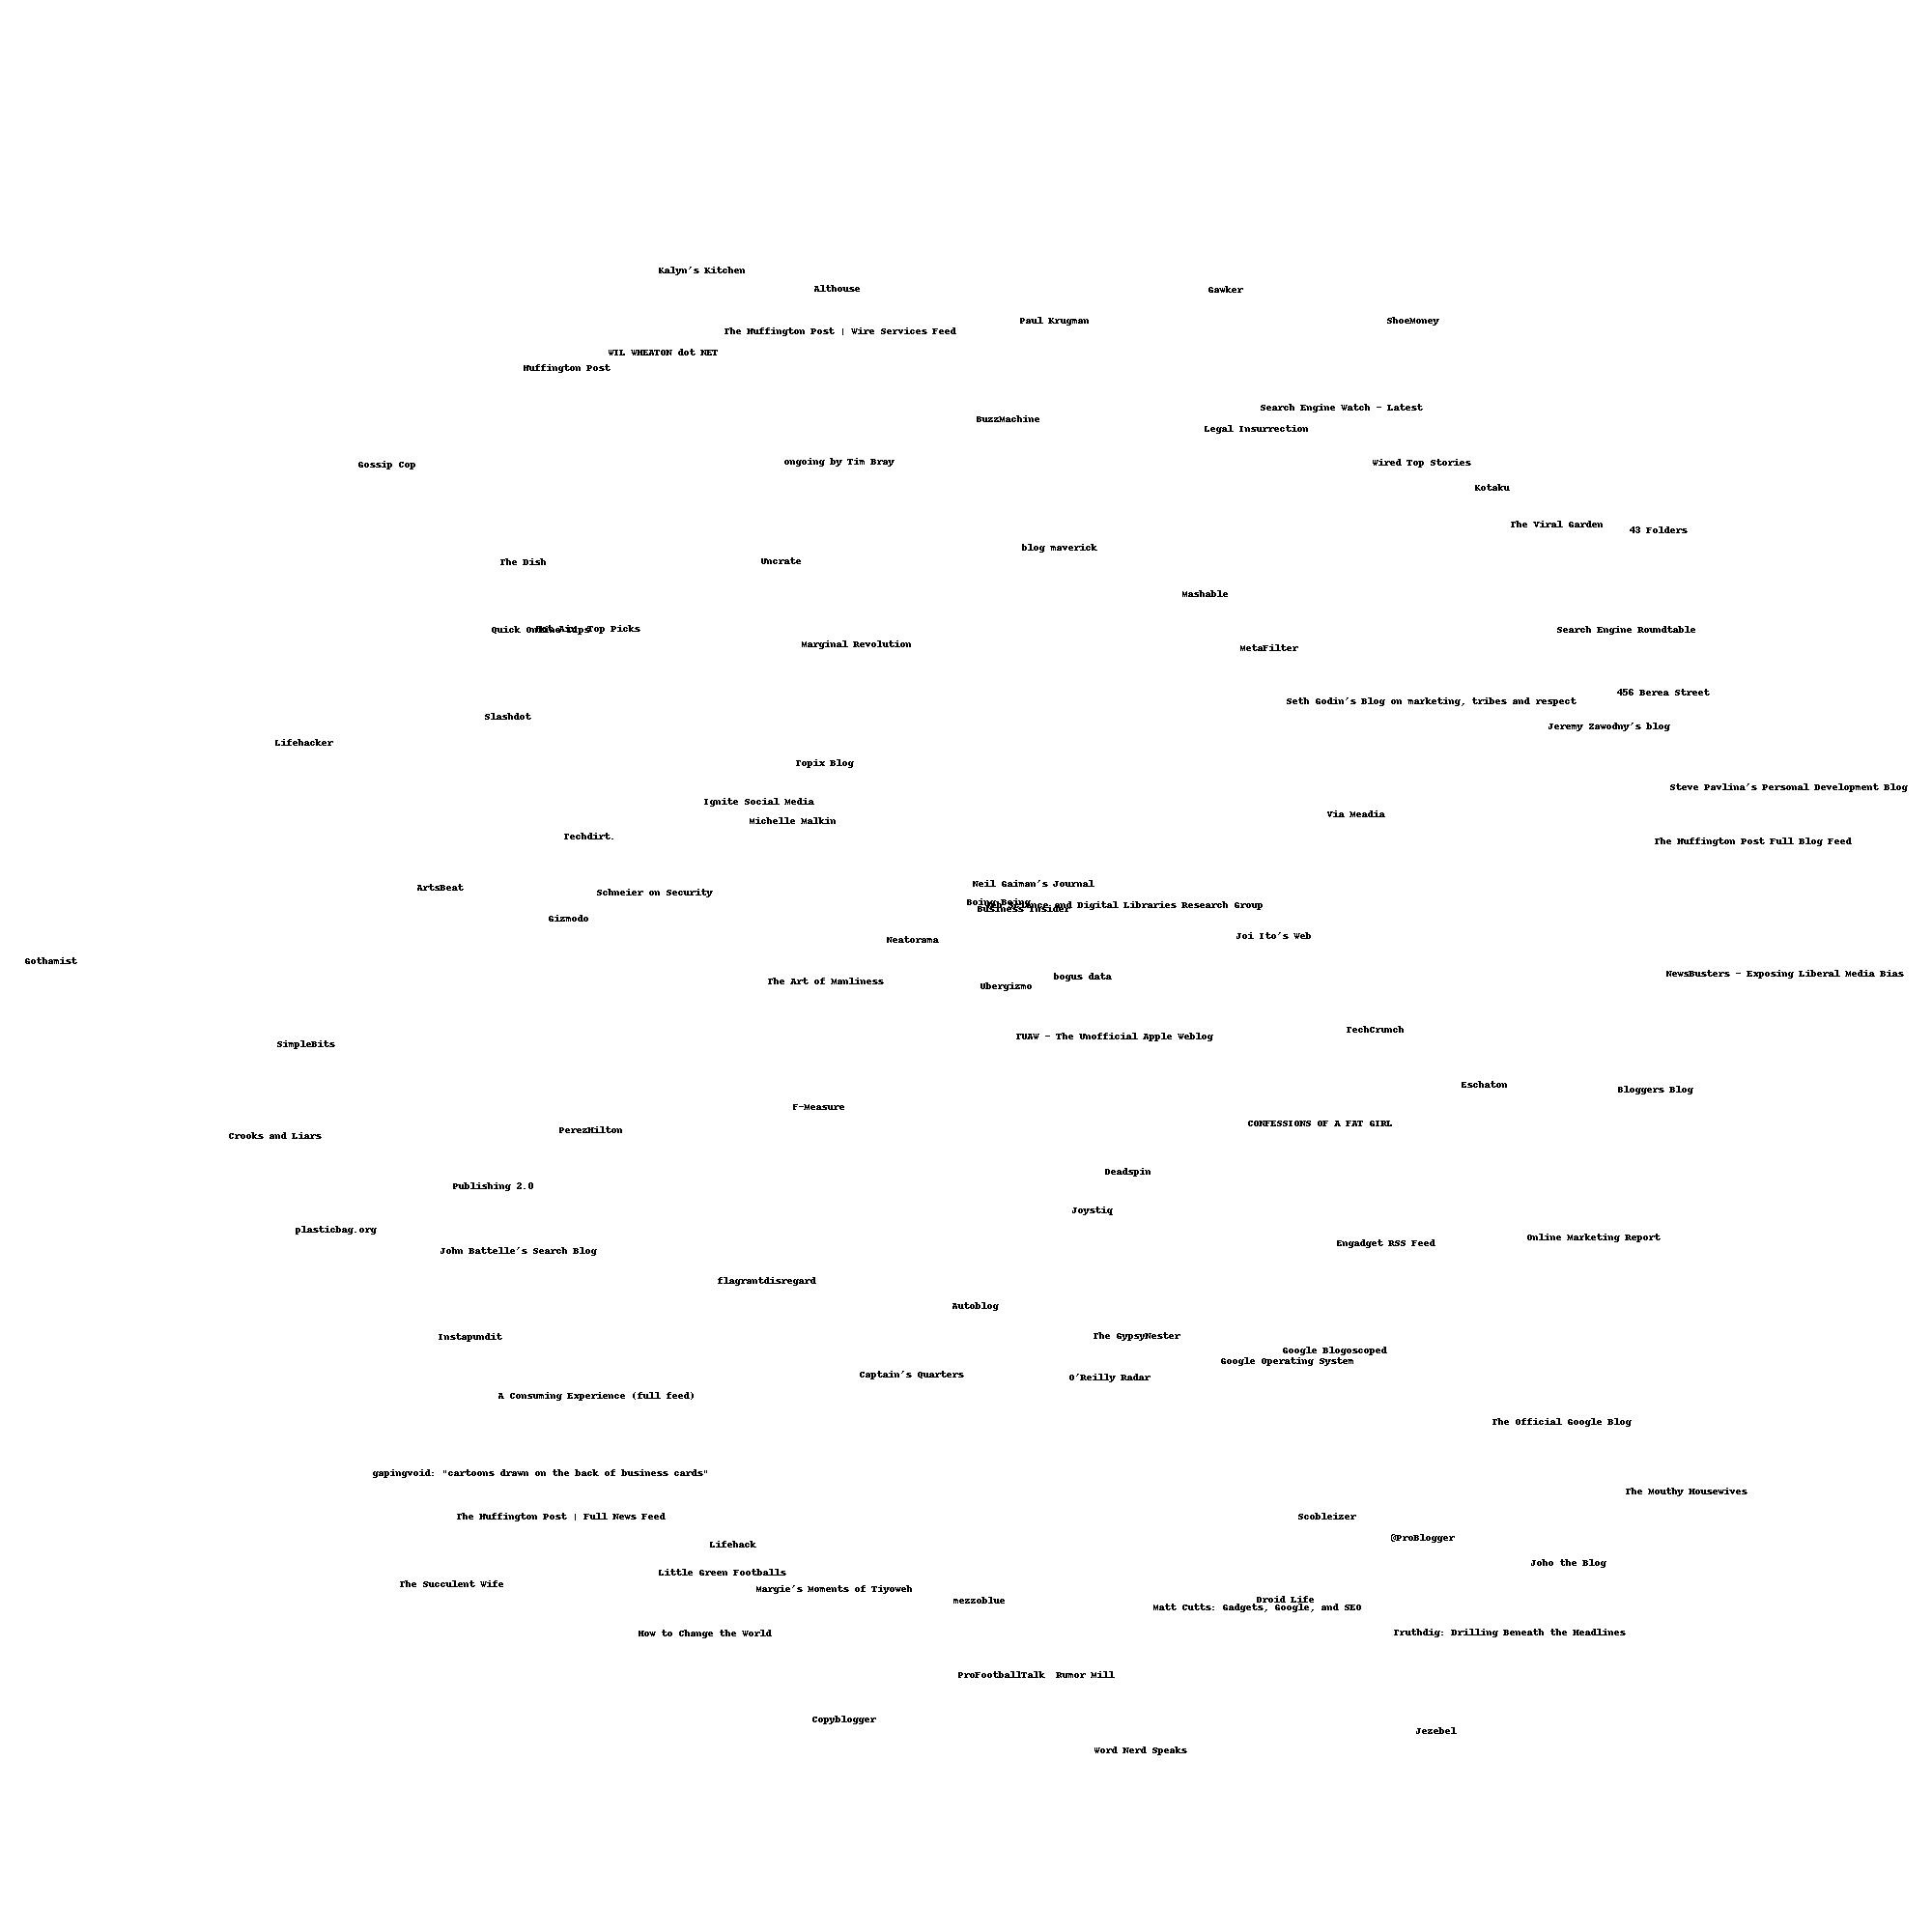
\includegraphics[scale=0.3]{blogs2d}
\caption{JPEG of the blogs using MDS}
\label{overflow}
\end{figure}
   
\end{answer}

\begin{answer}{5: Extra credit}

Fortunately, just two small changes to the code, in {\it generatefeedvector.py}, were sufficient to answer this question. The new code is stored in a new file called {\it generateq5.py}. The changes are: (1) for each blog, its total number of words is now computed. All other values needed to calculate {\it TFIDF} are already available from question 1, and (2) the final {\it TFIDF} value is computed and used instead of the original frequencies values to produce the final blog-term matrix. The new data file, which has the final blog-term matrix, is called {\it blogdataq5.txt} and it's already uploaded into our class repository. A copy of {\it cluster.py} is made and called {\it clusterq5.py} which will work to produce both JPEG and ASCII clustering format.

Figure 5 shows the JPEG dendrogram of how blogs are clustered based on {\it TFIDF} values:


\begin{figure}[ht!]
\centering
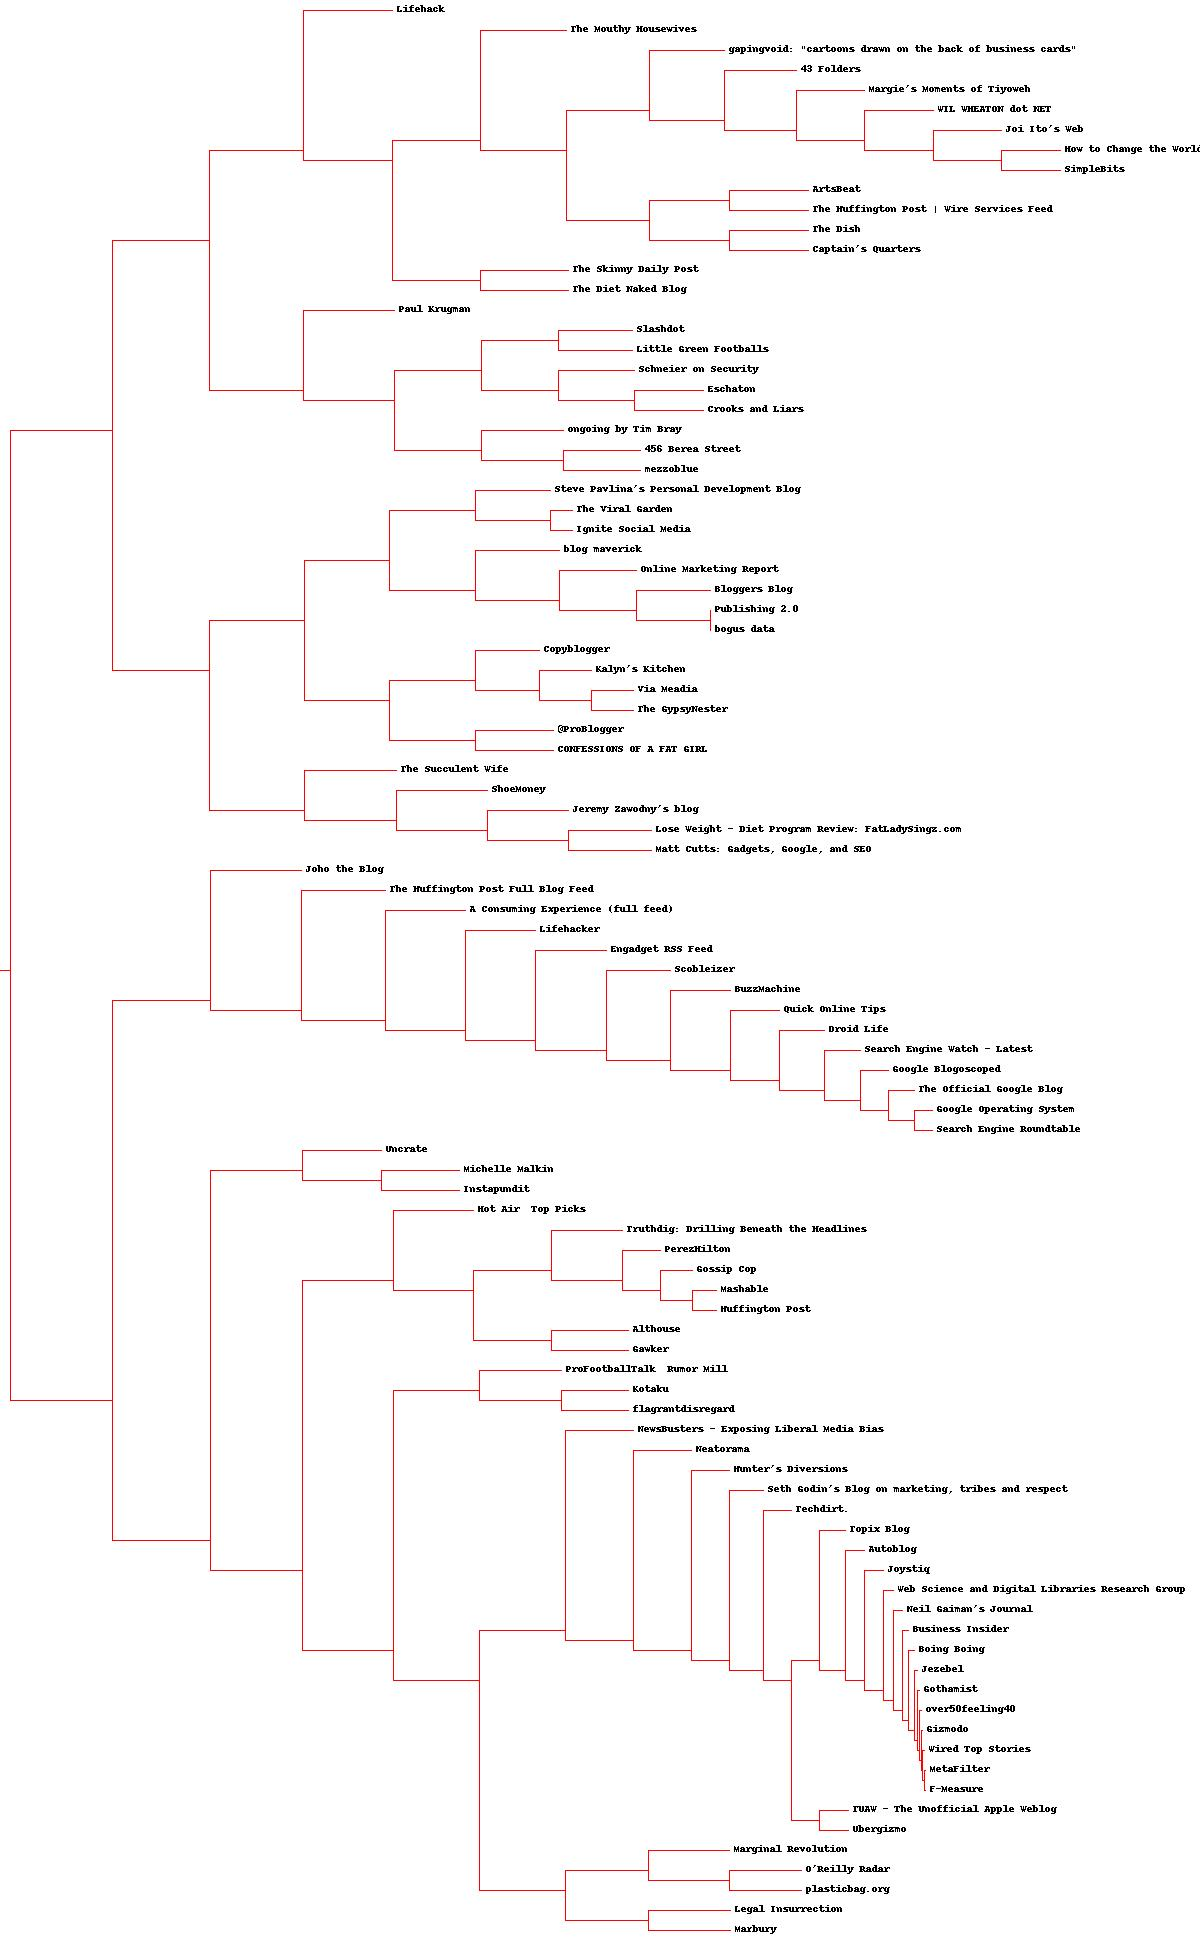
\includegraphics[scale=0.28]{blogclustq5}
\caption{JPEG dendrogram of the blog clusters based on TFIDF}
\label{overflow}
\end{figure}
 
When seeing the two JPEG figures, produced from question 2 and 5, I can not see big difference. For example, from question 2, the blog "Web Science and Digital Libraries Research Group" is placed at a level where the following blogs are placed below it: Business Insider, Boing Boing, Gizmodo, Gothamist, over50feeling40, Jezebel, Wired Top Stories, and F-Measure while ,from question 5, the same blog has the following blogs below it:                               Neil Gaiman's Journal, Business Insider, Boing Boing, Jezebel, Gothamist, over50feeling40, Gizmodo, Wired Top Stories, MetaFilter, and and F-Measure. In this case, only one blog (MetaFilter) has moved to join this sub-group in question 5 answer. In general, this may happen because of two reasons: first, computationally, the two mechanisms are different since one depends on the words frequencies while the other depends on the TFIDF values. Second, because the blogs are changing over time, running different algorithms at slightly different times may result in producing different clusters.



\end{answer}

\begin{thebibliography}{1}
\bibitem{one}
 On-line GitHub repository, 
{\tt \\https://github.com/nico/collectiveintelligence-book }.

\bibitem{two}
online Atom/RSS feed validation service, 
{\tt http://validator.w3.org/feed/}.


\end{thebibliography}
 

\end{document}
